\chapter{Identify ambiguous tasks}
\enlargethispage{3\baselineskip}

\begin{keypointstwomargins}{Identify ambiguous tasks}{-2cm}{-1cm}

        \textbf{Key points -- Identify ambiguous tasks}
        \begin{enumerate}[leftmargin=*]
        \item We know that datasets with better quality will lead to better models. It is famously a complicated task to explore big datasets and find ambiguous tasks in classical supervised setting. What can we do for crowdsourced datasets?
        \item While entropy or variance based methods in distribution votes are useful to retrieve tasks that lead to very noisy decisions, they are not fit in settings with few votes per tasks. And even less fitted to settings where a task can be labeled by a single worker. Can we still exploit these tasks?
        \end{enumerate}

        \textbf{Contributions -- Weighted Area Under the Margin}
        \begin{enumerate}[leftmargin=*,start=3]
        \item Following the literature on label noise, we adapt the AUM by \citet{pleiss_identifying_2020} into the AUMC and WAUM, two strategies to identify ambiguous tasks in datasets. The first is the baseline and directly falls back to the classical AUM using a majority vote. The WAUM introduces a trust score in the balance not to use poorly performing workers answers.
        \item We provide a simple guideline: pruning most ambiguous tasks from the dataset, and report computer vision classifier performance with and without pruning on simulated and three real datasets: \texttt{CIFAR-10H}, \texttt{LabelMe} and \texttt{Music}.
        \end{enumerate}

\end{keypointstwomargins}

\section{Do we know what is in our training sets?}
While our datasets are getting larger and larger every year, one question naturally arises: \emph{What is the quality of our training sets?}
Indeed, small datasets can easily be looked at, but thousands of images -- if not millions -- represent an herculean human work without assistance.

Data quality is linked with models performance \citep{budach2022effects}, looking for outliers to prune or weight differently during the learning procedure is not new \citep{angelova2004data}.
In this chapter, we first present the Area Under the Margin ($\AUM$): a statistic from \citet{pleiss_identifying_2020} that uses model iterates score prediction to detect unreliable training data points in the classically supervised learning setting.
Then, we propose to extend the $\AUM$ to the crowdsourcing setting with the Weighted Areas Under the Margin ($\WAUM$).
We show that the $\WAUM$ allows to identify ambiguous tasks in crowdsourced datasets, and pruning a portion of those tasks leads to better test performance overall.
We finish by discussing where do these tasks come from, going back to the dataset's creation and 

\subsection{Detect labeling errors in classical datasets}
% Cleanlab, confident learning, aum (litterature presentation and motivation mostly)
In classically supervised learning setting, training sets, tasks are paired up with a single label: $\mathcal{D}_\text{train}:=\{(x_i,y_i)\}_{i\in [n_\text{task}]}$.
This label has been assigned either automatically or via human decision.
Thus, the task might be mislabeled.
We can see a mislabeled task as a task that is difficult to classify for the classifier given this wrong label.
The $\AUM$ from \citet{pleiss_identifying_2020} allows us to identify tasks that are the most difficult to classify from the dataset.

More formally, the $\AUM$ of a task $(x_i,y_i)$ from a training set $\mathcal{D}_\text{train}$ given a classifier $\mathcal{C}$ and a number of training epochs $T>0$ is defined as:
\begin{equation}\label{eq:aum}
    \AUM(x_i, y_i; \mathcal{D}_\text{train}) = \frac{1}{T}\sum_{t=1}^T \left[\mathcal{C}^{(t)}(x_i)_{y_i} - \max_{k\neq y_i} \mathcal{C}^{(t)}(x_i)_k\right] \enspace.
\end{equation}
The $\AUM$ averages over time how far the score for the given class is from the most predicted other class by the classifier.
This is an average over time of the prediction margin.
It is classical to look at this margin in the literature to bound test error.
For example, \citet{bartlett1998boosting} showed that test error is dependent of the margin's distribution over the training set, even with zero error reached during training. 
However, the $\AUM$ does not consider the margin given a trained classifier, but looks at the early dynamics in the training procedure.

\begin{figure}[thb]
\begin{minipage}{.45\linewidth}
\centering
\subfloat[Mislabeled image: $\AUM\ll 0$]{\label{mnist:low}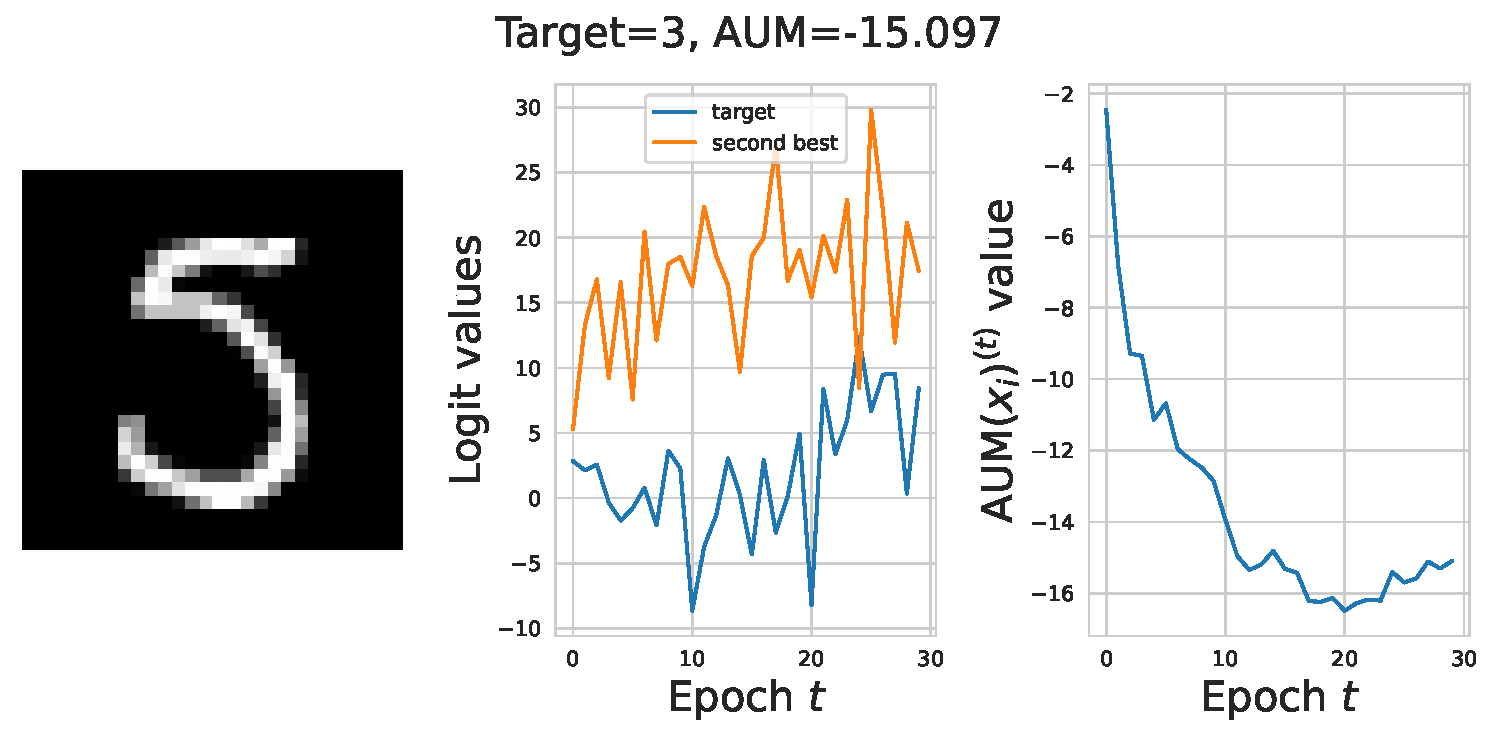
\includegraphics[width=\textwidth]{chapters/images/low_aum_mnist.pdf}}
\end{minipage}%
\hfill
\begin{minipage}{.45\linewidth}
\centering
\subfloat[Correct label: $\AUM\gg 0$]{\label{mnist:high}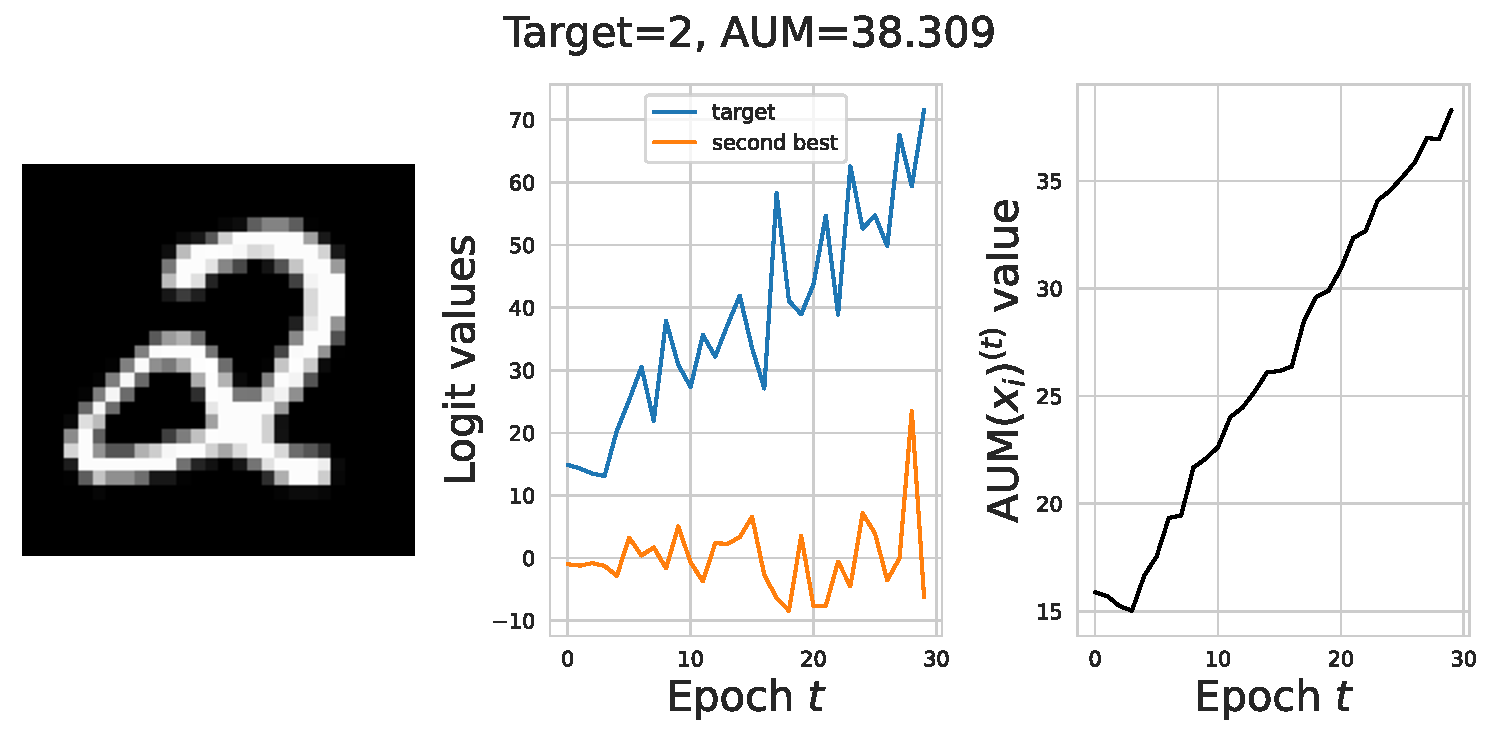
\includegraphics[width=\textwidth]{chapters/images/high_aum_mnist.pdf}}
\end{minipage}\par\medskip
\begin{center}
\subfloat[Confusion: the image is either a four or a nine cut-out with true label $y_i^\star=9$, the $\AUM$ is closer to zero indicating high ambiguity in learning classes]{\label{mnist:mid}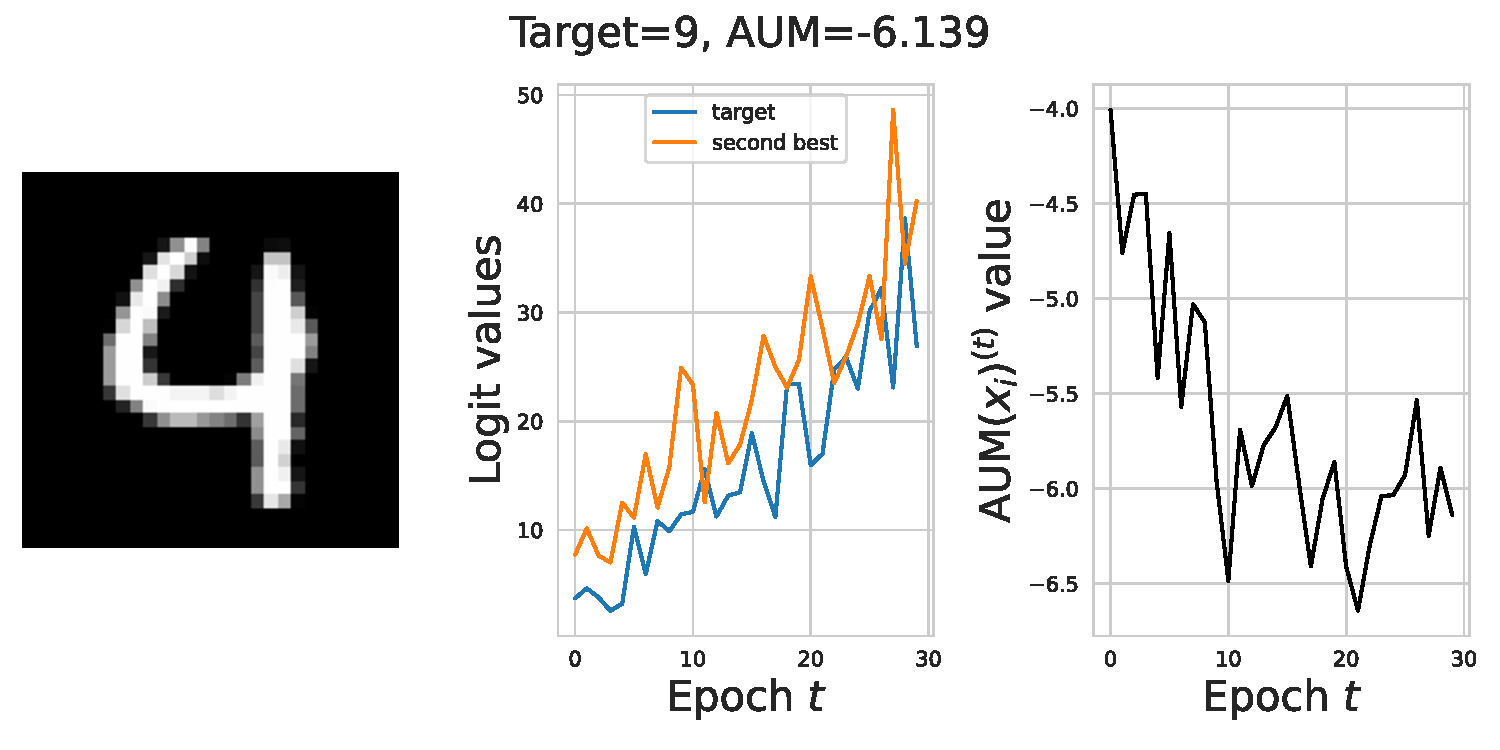
\includegraphics[width=.6\textwidth]{chapters/images/mid_aum_mnist.pdf}}
\end{center}
\caption{Three examples from the MNIST dataset to illustrate the behavior of the $\AUM$: if the sample is mislabeled the $\AUM$ is low as the classifier disagrees with the given label. Note that if $T>0$ is too high the memorization kicks-in and the $\AUM$ increases again. When the sample is correctly labeled the $\AUM$ increases over training. When the sample is ambiguous, the $\AUM$ is closer to $0$. Results are from a 2-layer convolution network with max-pooling. Training is done in $T=30$ epochs using Adam optimizer with learning rate set to $0.01$ and batches of $100$ samples.}
\label{fig:mnist_aum}
\end{figure}

This early dynamic, and by association the hyperparameter $T>0$, is necessary as it is well known that modern neural networks classifier are able to memorize the data and even classify correctly random tasks because of the hyperparametrization \citep{maennel2020neural}.
The memorization is a necessary phenomenon for training a neural network: we need the classifier to memorize patterns.
But what we wish to consider the least in the $\AUM$ is the unintended memorization \citep{maennel2020neural} that can happen early and is difficult to temper -- even with strategies like dropout or weight decay.
And in \citet{zhang2021understanding}, they show -- among other results -- that true labels are learned faster than random labels by neural networks classifier.
This early training dynamic in the prediction logits can thus be used as a proxy to identify possible mislabeled data.

Note that there exist other algorithms to learn from mislabeled data, such as Confident Learning \citep{northcutt_confident_2021} using by \texttt{CleanLab}\footnote{\url{https://cleanlab.ai/}}.
Confident Learning does not correct the label nor does it re-weight the data.
It estimates the joint distribution between the given and unknown latent labels with class-conditional noise and then prune samples by-class with threshold the average predicted probability for the samples in the given class.
With the $\AUM$, we can also correct the label during training -- even though we will not consider this application for this work.

% (results of the litterature in classical supervised setting)
% Examples on mnist, cifar10, imagenet

\section{The WAUM: extending the AUM to the crowdsourcing setting}

While the $\AUM$ shows results of identifying different types of samples difficulty by averaging the margin during $T>0$ training epochs, there is no direct way to apply it to the crowdsourcing setting.
Indeed, the $\AUM$ needs, by definition, a hard label $y_i$ to consider the assigned-label score $\mathcal{C}(x_i)_{y_i}$ and also to consider the second biggest score for a class different than $y_i$.
In the crowdsourcing setting however, there is no direct hard label $\hat y_i$ from the multiple answers $\{y_i^{(j)}\}_{j\in\mathcal{A}(x_i)}$ to a task $x_i$.

A naive transformation to apply the $\AUM$ in a crowdsourcing setting is to consider the majority voting aggregation. \Cref{eq:aum} simply becomes:
\begin{equation}\label{eq:aum_mv}
    \AUM \mathrm{C}\left(x_i, \{y_i^{(j)}\}_j\right) := \frac{1}{T}\sum_{t=1}^T \left[\mathcal{C}^{(t)}(x_i)_{\hat y_i^{\mathrm{MV}}} - \max_{k\neq \hat y_i^{\mathrm{MV}}} \mathcal{C}^{(t)}(x_i)_k\right] \enspace.
\end{equation}
The $\AUM\mathrm{C}$ strategy lacks the worker abilities and task difficulty.
There is no worker-specific margin, in fact the MV aggregation strategy removed the worker-specific information from the $\AUM$.
In the following, we introduce the $\WAUM$: a statistic that generalizes the $\AUM$ to the crowdsourcing setting by aggregating worker-specific margins into a weighted average to consider both worker abilities and task difficulty.

\subsection{Definition and construction of the WAUM}
% Explain weights choice and variations
Given a number of training epochs $T>0$ and a classifier $\mathcal{C}$ for a crowdsourced training set $\mathcal{D}_\text{train}$, we write the $\WAUM$ as a weighted average of worker specific $\AUM$.
More formally:
\begin{equation}\label{eq:waum}
    \WAUM\left(x_i;\mathcal{D}_\text{train}\right):=
\end{equation}

\subsection{Evaluating the WAUM}

\subsection{Results on simulated datasets}
Circles (good) + Two moons (not all ambiguities are to be removed)

\subsection{Results on datasets with tasks available}
CIFAR-10H + LabelMe + Music

\subsection{Where can these errors come from? Going back to the dataset creation and discussion}
(motivation + transition for the need of WAUM)
Example of CIFAR-10 to CIFAR-10H. The lack of explainations in crowdsourcing. Recent conference (Neurips) ask for detailed explainations now for new datasets, but crowdsourced data is often not released.
